\section{Set-Up}
For the study of the QHE a two-dimensional or quasi two-dimensional system is needed.
In this experiment a quantum well is created by confining electrons in a thin layer of HgTe between
two layers of HgCdTe. Because of the smaller bandgap of HgTe compared to HgCdTe a quantum well is formed. 
At low temperatures (liquid helium), all electrons are located in the lowest energy level of the 
two dimensional quantum well. This creates a confinement in the layer stacking direction.
Inside the quantum film of HgTe, the electrons form a two-dimensional electron gas (2DEG) with high mobility.
All measurements are done in a variable temperature insert (VTI), which allowes to cool the sample down to a
range between roughly $4.2\,\text{K}$ and $1.5\,\text{K}$ by evaporating He at different pressures. The sample is designed in a common Hall bar geometry,
with in total $8$ contacts on the edges with a additional pair for the Gate voltage (see fig.\,\ref{fig:HallBar})
\begin{figure}[h]
    \centering
    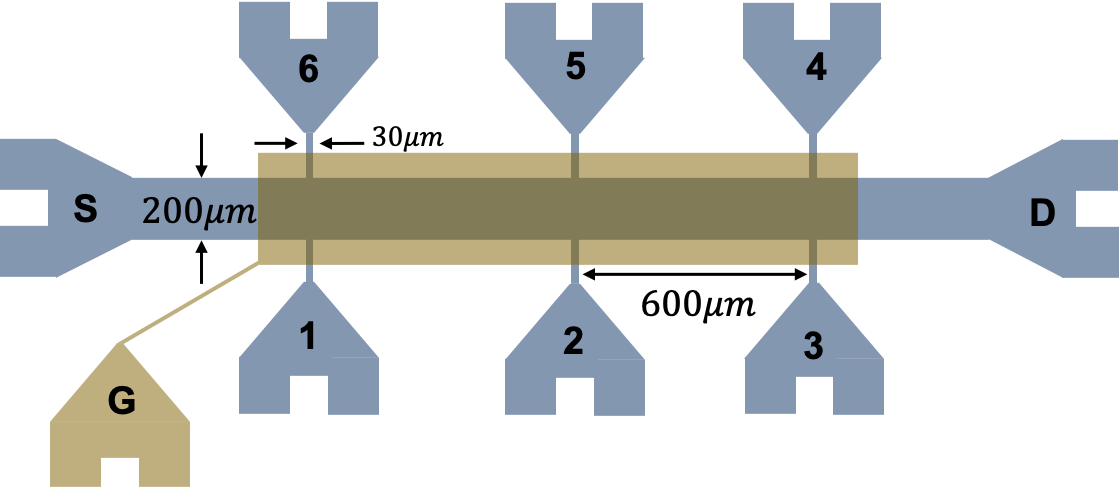
\includegraphics[width=0.45\textwidth]{../Images/HallBar.png}
    \caption{Schematic of the Hall bar geometry. The contacts are labeled with "S" for source, "D" for drain,
    "G" for gate. Contacts $4$ and $6$ are used for the measurement of the longitudinal resistance 
    and contacts $3$ and $4$ are used for the measurement of the transversal resistance.}
    \label{fig:HallBar}
\end{figure}
An AC voltage is applied between source and drain to control the longitudinal current $I$
flowing through the sample. $I$ can be measured via the voltage drop $U_\text{I}$ over a known resistor $(R_\text{S}=4.982\pm0.0005)\,\text{k}\Omega$, 
which is connected in series to the source contact. $U_\text{I}$ is measured with a Lock In amplifier 
\emph{Stanford Research Systems SR510}. Contacts $3$ and $4$ are used to measure the hall voltage $U_\text{Hall}$, which
is measured with a second Lock In amplifier of the same type. Contacts $4$ and $6$ are used to measure
the longitudinal Voltage $U_\text{xx}$, which is measured with a third Lock In amplifier \emph{Stanford Research Systems SR530}.
All Lock In amplifiers use a phase sensitive amplification approach by filtering the the noise through multiplying the signal
with a $13\,\text{Hz}$ reference signal. Moreover, the data is integrated over a period of $3\,\text{s}$ and measured with a sensitivity of $1\,\text{mV}$.
The hall bar sample has a width of $200\,\mu\text{m}$ and a length of $1.2\,\text{mm}$, which can be seen in fig.\,\ref{fig:HallBar}.
For observation of the hall effect, a magnetic field $B$ is applied perpendicular to the plane of the sample.
The magnetic field is generated by a superconducting NbTi solenoid, which is cooled with liquid helium and can
be precisely controlled by the current flowing through the magnet. The flux density $B$ is read out as a voltage
$U_\text{B}$ with $U_\text{B}=10\,\text{V}$ corresponding to $9\,\text{T}$. The temperature of the sample is measured
via the voltage drop over a "Alan Bradley" resistor $R_\text{AB}=100\,\Omega$ using a \emph{Keithley 160B} digital multimeter and a constant current of $10\mu\text{m}$.
Acting as a resistive thermometer the carbon resistor is located with the sample inside the VTI and is calibrated for the used temperature range.
The conversion of Voltage to Temperature is done with the calibration table \cite{ExperimentDescription}.


